\subsection*{Tilpasning af træningsniveau}
Førend en træning kan påbegyndes, tilpasses træningsniveauet den enkelte bruger. Tilpasning af træningsniveauet er inddelt i fire boundarys. Disse håndteres af en samlet controller, hvilket fremgår af \autoref{fig:DesignTilpasning}.

\begin{figure} [H]
\centering
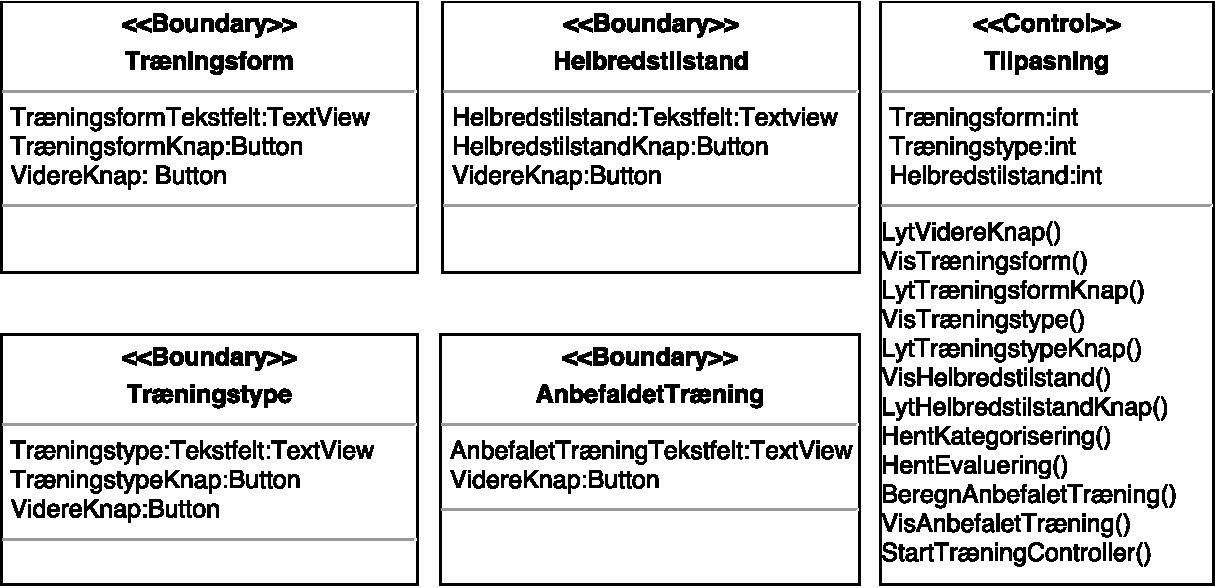
\includegraphics[width=1\textwidth]{figures/MVC/MVCTilpasning}
\caption{Designklasser for tilpasning af træningsniveau. Til venstre ses de fire boundarys for henholdsvis Træningsform, Træningstype, Helbredstilstand og AnbefaletTræning. Til højre fremgår den tilhørende controller.}
\label{fig:DesignTilpasning}
\end{figure}

\noindent
Der er opstillet grænseflader for tilpasning af træning, hvilket omfatter \textit{Træningsform}, \textit{Træningstype}, \textit{Helbredstilstand} og \textit{AnbefaletTræning}. Der er til hver grænseflade opstillet tekstfelter af typen TextView og knapper af typen Button.   

Den tilhørende controller til de ovenstående boundarys lagrer den angivne træningsform, træningstype samt helbredstilstand  i entityen, KonditionResultater, således disse senere kan sendes til databasen efter endt træning. Der er opstillet tilhørende attributter og metoder, herunder Vis, Lyt, Hent, Beregn og Start. Metoderne henter og beregner i forhold til definerede inputsparametre. Efter inputsparametre er der angivet, hvorvidt der returneres en værdi.

I sammenspil med designklasserne er der udarbejdet et sekvensdiagram, hvilket fremgår af \autoref{fig:SEKTilpasning}. 

\begin{figure} [H]
\centering
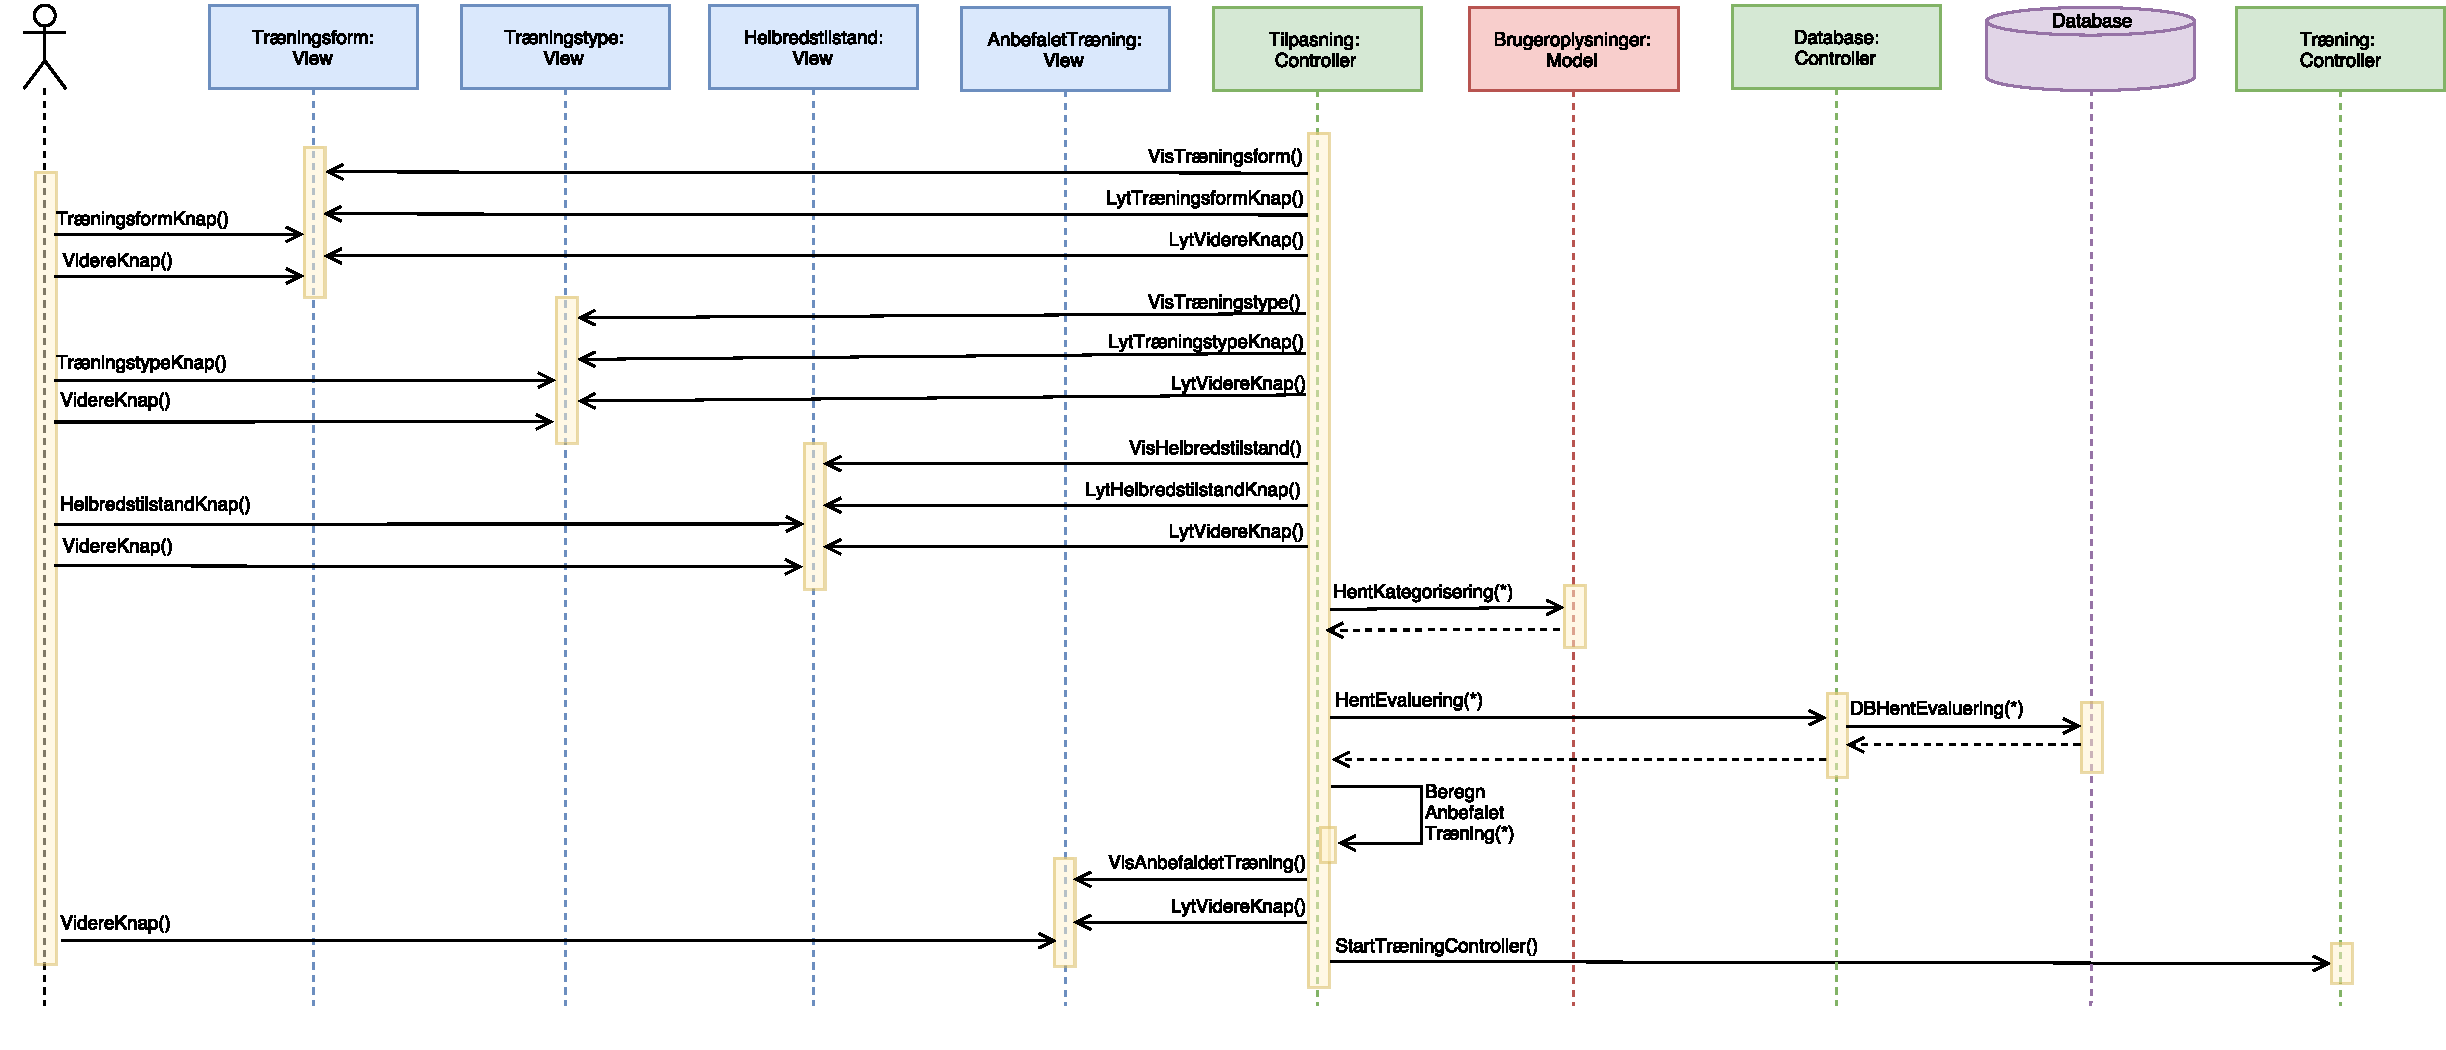
\includegraphics[width=1.55\textwidth, angle=90]{figures/Sek/SEKTilpasning}
\caption{Sekvensdiagram for tilpasning af træningsniveau.}
\label{fig:SEKTilpasning}
\end{figure}

\noindent
Den første grænseflade, som vises, er \textit{Træningsform}. Denne grænseflade indeholder et tekstfelt, der beskriver, hvad brugeren skal angive. Dertil er der opstillet en TræningsformKnap, hvor brugeren kan vælge mellem konditionstræning, styrketræning eller vejrtrækningsøvelser. Når der er angivet træningsform, trykker brugeren på VidereKnap, hvorefter \textit{Tilpasning}-controlleren viser grænsefladen for valg af \textit{Træningstype}. Brugeren skal her angive træningstype ud fra tre forskellige muligheder. Dette vil for eksempel ved konditionstræning være gå, løbe eller cykle. Brugeren bekræfter valget ved at trykke på VidereKnap, hvorefter controlleren viser grænsefladen for \textit{Helbredstilstand}. Helbredstilstanden angives og bekræftes ved at trykke på VidereKnap. Herefter kaldes set-metoden fra modellen \textit{KonditionResultater}, hvori type og helbredstilstand gemmes. Controlleren henter kategoriseringen ved brug af get-metoden fra modellen \textit{Brugeroplysninger} og henter efterfølgende tidligere evaluering fra \textit{Database} via \textit{Database}-controlleren, hvis der eksisterer en tilhørende evaluering. 
Efterfølgende beregner \textit{Tilpasning}-controlleren anbefalet træningsniveau og viser dette på grænsefladen for \textit{AnbefaletTræning}. Brugeren kan herefter trykke på VidereKnap, hvis denne trykkes på, startes \textit{Træning}-controlleren. 
